\subsection{From Theory to Practice}

\newsavebox\abstractionbox
\begin{lrbox}{\abstractionbox}
\pgfmathsetseed{42}%
\begin{tikzpicture}[line cap=round]
   \pgfonlayer{foreground}
   \draw[Kite-Kite,very thick] (0,3.5) node[below right,yshift=1mm] {\(x(t)\)} |- (8,0) node[above left] {\(t\)}; % time vs. x at tat time
   \endpgfonlayer
   \colorlet{@}{gray}
   \draw[very thick,@] (0,1) plot [smooth] coordinates {(0,1) (1,2) (2,1) (3,2) (4,1) (5,2) (6,1) (7,2) (8,1)}; % x(t)
   \draw[very thick,@] (0,0) plot [smooth] coordinates {(0,0) (1,1) (2,2) (3,2) (4,2.5) (5,2.5) (6,.5) (7,.6) (8,.6)}; % x(t)
   \draw[very thick,@] (0,1.5) plot [smooth] coordinates {(0,1.5) (1,2) (2,2.5) (3,2) (4,2) (5,2.5) (6,2.5) (7,2) (8,2.5)}; % x(t)
      \foreach \i in {0,...,5} {
         \pgfmathsetmacro{\randA}{rnd*0.33}
         \pgfmathsetmacro{\randB}{rand*0.5}
         \pgfmathsetmacro{\randC}{rand*0.4}
         \draw[gray] (0,1.5+\randA) plot [smooth] coordinates {(0,1.5+\randA) (1,2-\randB) (2,2.5-\randA) (3,2-\randB) (4,2+\randA) (5,2.5) (6,2.5+\randA) (7,2-\randA) (8,2.5+\randB)} node[inner sep=0pt] (a-\i) {};
         \draw[gray] (0,0+\randA) plot [smooth] coordinates {(0,0+\randA) (1,1-\randB) (2,2-\randB) (3,2+\randC) (4,2.5-\randA) (5,2.5-\randB) (6,.5+\randC) (7,.6+\randB) (8,.6+\randC)} node[inner sep=0pt] (b-\i) {};
         \draw[gray] (0,1+\randB) plot [smooth] coordinates {(0,1-\randC) (1,2-\randB) (2,1+\randB) (3,2-\randA) (4,1+\randA) (5,2-\randB) (6,1) (7,2-\randC) (8,1+\randA)} node[inner sep=0pt] (c-\i) {};
      }
   % fit to all nodes to get the bounding box
   \node[fit=(a-0) (a-1) (a-2) (a-3) (a-4) (a-5) (b-0) (b-1) (b-2) (b-3) (b-4) (b-5) (c-0) (c-1) (c-2) (c-3) (c-4) (c-5),inner sep=0pt] (big-ghost) {~};
      % \draw[decorate,thick,decoration={brace,amplitude=5pt,raise=2pt},gray] (big-ghost.north east) -- (big-ghost.south east);
   \pgfonlayer{background}
   \pgfinterruptboundingbox
   \fill[red,opacity=.175,even odd rule] plot [smooth] coordinates {(0,0) (1,0.4) (2,0.5) (3,1) (4,.8) (5,1) (6,.1) (7,0.2) (8.03,.2) (8.03,3) (7,2.8) (6,3) (5,2.95) (4,2.85) (3,2.75) (2,2.65) (1,2.5) (0,2) } -- cycle (6,1.85) circle[radius=4mm]; 
   \endpgfinterruptboundingbox
      \node (@b1) at (6,1.85) {\small\faBug};
      \node (@b2) at (3,.35) {\small\faBug};
      \node (@b3) at (7,2.5) {\small\faBug};
      \node[above left=-1mm,green] at(@b2.south east) {\scriptsize\faCheck};
      \node[above left=-1mm,green] at(@b1.south east) {\scriptsize\faCheck};
      \node[above left=-1mm,yshift=1pt,orange] at(@b3.south east) {\scriptsize\faQuestion};
   \endpgfonlayer
   \path[use as bounding box] (0,0) rectangle (8,3.5);
\end{tikzpicture}
\end{lrbox}

\begin{frame}{What we have\ldots}
\frametitle<-8>{\strut What we have\ldots}%
\frametitle<9->{\strut\textcolor{gray}{What we have\ldots~}Theory}%
\begin{uncoverenv}<2->  
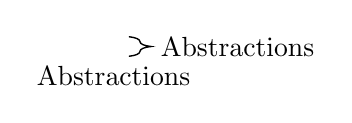
\begin{tikzpicture}[baseline={([yshift=-.5ex]current bounding box.center)},line cap=round]
   \tikzset{@/.style={opacity=1}}
   \def\scaler{1}
   \only<4->{\def\scaler{0.5}\tikzset{@/.style={opacity=.5,scale=.5,every node/.style={transform shape}}}}
   \scope[transparency group, @]
   \node (@) at (0,0) {\usebox\abstractionbox};
   \onslide<3>{
   \draw[decorate,thick,decoration={brace,amplitude=8pt*\scaler,raise=2pt},line width=0.5pt*\scaler] (@.north east) to[edge node={node [right=3.5mm] {Abstractions}}] (@.south east);
   }
   \onslide<4->{%
      \node[below] at(@.south) {Abstractions};
   }
   \endscope
\end{tikzpicture}\qquad
\begin{uncoverenv}<5->
\begin{tikzpicture}[r/.style={rectangle,draw,minimum width=2cm,minimum height=1cm,rounded corners=1pt},baseline={([yshift=-.5ex]current bounding box.center)},line cap=round]
   \tikzset{@/.style={opacity=1}}
   \def\scaler{1}
   \only<7->{\def\scaler{0.5}\tikzset{@/.style={opacity=.5,scale=.5,every node/.style={transform shape}}}}
   \scope[@]
   \scope[black!25!white,scale=.7,every node/.style={transform shape}]
   \node[r] (@) at(0,0) {};
   \node[r, below left=1cm] (@a) at(@.south) {};
   \node[r, below right=1cm] (@b) at(@.south) {};
   \node[r,below=1cm] (@c) at(current bounding box.south) {};
   \draw[-Kite] (@) -- (@a.north);
   \draw[-Kite] (@) -- (@b.north);
   \draw[-Kite] (@a.south) -- (@c);
   \draw[-Kite] (@b.south) -- (@c);
   \endscope
   \node[align=center,text width=4.5cm] at(current bounding box.center) {\small%
\begin{align*}
   \mathbf{In}_n &= (\mathbf{Out}_n - \mathbf{Kill}_n) \cup \mathbf{Gen}_n \\
   \mathbf{Out}_n &= \begin{cases}
      \mathbf{BI} & n \text{~is End} \\
      \bigcup\limits_{m \in \text{succ}(n)} \mathbf{In}_m & \text{otherwise}
   \end{cases}
\end{align*}
   };
   \onslide<6->{
      \node[below=5mm] at(current bounding box.south) {Data Flow Analysis};
   }
   \endscope
\end{tikzpicture}
\end{uncoverenv}\qquad
\hspace*{4.5em}\onslide<8->{\large\ldots}
\end{uncoverenv}
\end{frame}

\newsavebox\MagicPenguin
\savebox\MagicPenguin{\tikz{\pingu[witch hat,eyes wink,wings wave,bee,blush,santa beard]}}
\newsavebox\MagicPenguinTwo
\savebox\MagicPenguinTwo{\tikz{\pingu[witch hat,eyes shiny,bee,santa beard]}}
\begin{frame}{What we want\ldots}
   \frametitle<1>{\strut What we want\ldots~}%
   \frametitle<2->{\strut\textcolor{gray}{What we want\ldots~}Tools}%
   \centering\kern1.345em
   \begin{uncoverenv}<3->
   \begin{tikzpicture}[o/.style={outer sep=0pt,inner sep=0pt},line cap=round,Rect/.style={draw,rectangle,rounded corners=3pt,inner sep=4pt,outer sep=1mm},draw=gray,every path/.append style={thick}]
      \node[o] (@) at (0,0) {\usebox\CodeFile};
      \pgfonlayer{background}
      \scope[transparency group,opacity=.4]
      \node[o,rotate around={-30:(@.south east)},anchor=south east] at(@.south east) {\usebox\CodeFile};
      \node[o,rotate around={-12:(@.south east)},anchor=south east] at(@.south east) {\usebox\CodeFile};
      \endscope
      \endpgfonlayer
      \node[below] at(@.south) {\small Project};
      \onslide<3->{
         \node[right=1.33cm,Rect,minimum width=4.5em] (@magic) at(@.east) {~\vphantom{Magic}{\only<8->{\only<9->{\color{gray!34}}\clap{Magic}}}\only<9->{\clap{\kern-.8pt\textbf{Tools}}}~\null};
         \draw[-Kite] ([xshift=5mm]@.east) -- (@magic.west);
      }
      % and how can we achieve that?... magic :sparkles: but as there is no magic, we need tools... and algorithms
      \onslide<8->{
         \node[above right,xshift=1.3mm] at(@magic.north west) {\scalebox{.45}{\only<-8|handout:0>{\kern-8.5pt\usebox\MagicPenguin}\only<9->{\usebox\MagicPenguinTwo}}};
      }
      \coordinate (@) at(@magic.east);
      \foreach[count=\i] \usecase/\targeti in {Security/4, Maintenance/5, Comprehension/6, Optimization/7, Usability/7, \ldots/7} {
      \pgfmathsetmacro\rot{-11*\i+38.75}
         \onslide<\targeti->{
            \node[right=1cm,Rect,rotate around={\rot:([xshift=-9mm]@.east)},minimum width=8em,fill=white] (@uc-\i) at (@.east) {\strut\usecase};
            \draw[-Kite,sharp corners] (@.east) -- ++(4.2mm,0) [rounded corners=1pt] arc (0:\rot:9mm) -- (@uc-\i.west);
         }
      }
      \onslide<11->{
         \scope[gray]
         \node[right] at (@uc-1.east) {\small injections, leaks,~\ldots};
         \node[right] at (@uc-2.east) {\small code clones, deprecation,~\ldots};
         \node[right] at (@uc-3.east) {\small documentation, structure,~\ldots};
         \node[right] at (@uc-4.east) {\small better algorithms, memoization,~\ldots};
         \node[right] at (@uc-5.east) {\small color deficiency, size,~\ldots};
         \node[right] at (@uc-6.east) {\small \only<-11|handout:0>{\ldots}\only<12->{architecture recovery, refactoring,~\ldots}};
         \endscope
      }
      \onslide<13->{
         \draw[Kite-] (@magic.south) -- ++(0,-.66) node[below,align=center,font=\footnotesize] {SonarQube\rlap{\textsuperscript{1}}, Teamscale\rlap{\textsuperscript{2}},\\lintr\rlap{\textsuperscript{3}}, CodeQL\rlap{\textsuperscript{4}}, \ldots};
      }
   \end{tikzpicture}

   \begin{tikzpicture}[overlay,remember picture]
      \onslide<10->{%
         \node[above=9mm,lightgray] at(current page.south) {\footnotesize\enquote{Any sufficiently advanced technology is indistinguishable from magic.} --- Arthur C. Clarke};% 3rd law
      }
      \only<13->{\node[bottom note,above right,yshift=5mm] at(current page.south west) {%
         \textsuperscript{1}\,\href{https://www.sonarsource.com/}{sonarsource.com}, \textsuperscript{2}\,\href{https://teamscale.com/}{teamscale.com}, \textsuperscript{3}\,\href{https://lintr.r-lib.org/}{lintr.r-lib.org}, \textsuperscript{4}\,\href{https://codeql.github.com/}{codeql.github.com}%
      };}
   \end{tikzpicture}
   % TODO: tool examples
   % rather list concrete problems than tools
\end{uncoverenv}
\end{frame}


\begin{frame}{\strut What do they\ldots~do?}
% they take input, textual, syntactical, semantic (call graphs, pdg, ...), metadata, historical information, requirements, annotations (types, contracts), ...
\hspace*{-3.5mm}
\begin{tikzpicture}[o/.style={outer sep=0pt,inner sep=0pt}]
   \onslide<2->{%
      \node[o] (@) at (0,0) {\usebox\CodeFile};
      \node[above=2.5mm,xshift=1.15mm,gray] at(@.north) {\tiny They take \textbf{\normalsize Input}};
   }
   \pgfonlayer{background}
   \onslide<2->{%
   \scope[transparency group,opacity=.4]
   \node[o,rotate around={-30:(@.south east)},anchor=south east] at(@.south east) {\usebox\CodeFile};
   \node[o,rotate around={-12:(@.south east)},anchor=south east] at(@.south east) {\usebox\CodeFile};
   \endscope}
   \endpgfonlayer
   \begin{uncoverenv}<3->
   \coordinate (@) at(@.east);
   \foreach[count=\i] \usecase/\targeti in {{\raisebox{1pt}{Textual}}/4,Syntactical/5, Semantical/6, Historical/7, Annotated/8, {\only<-9|handout:0>{\ldots}\only<10->{\raisebox{-3pt}{Metadata,~\ldots}}}/9} { % program spectra, hardware, contexts, ...
   \pgfmathsetmacro\rot{-24*\i+66}
      \onslide<\targeti->{
         \path ([xshift=.5mm]@.east)++(\rot+10:1mm) coordinate (@a);
         \fill[opacity=.18,gray] (@a.east) -- ++(\rot:1.5cm) arc (\rot:\rot+20:1.5cm) -- cycle;
         \draw[thick,gray] (@a.east)++(\rot:1.5cm) arc (\rot:\rot+20:1.5cm);
         \path (@a.east) -- ++(1.05*\rot+10:1.6cm) node[right,font=\small,darkgray] (@uc-\i) {\vphantom{a}\smash{\usecase}};
      }
   }
   \node[above=1.65mm,xshift=1mm,gray] at(current bounding box.north) {\tiny And use \textbf{\normalsize Perspectives} \rlap{(often combined)}};
   \end{uncoverenv}
   \onslide<11->{%
      \draw[Kite-,gray] ([xshift=6.25mm,yshift=-1mm]current bounding box.south) to[out=-90,in=0] ++(-4.5mm,-5mm) node[below left,yshift=.42\baselineskip,align=right,text width=2.5cm,font=\tiny] {Some of those are the result of other static or dynamic analyses};
   }
   \begin{uncoverenv}<12->
      \node[right,yshift=-2mm,xshift=1cm,align=left,font=\small,darkgray,text width=3.25cm] (@techn) at(current bounding box.east){{\onslide<13->{\subnode{tc-search}{Text/Code Search}\strut}}~\\[4mm]\strut{\onslide<14->{\subnode{clustering}{Clustering}}}~\\[4mm]\strut{\onslide<15->{\subnode{ai}{Abstract Domains}}}~\\[4mm]\strut{\onslide<16->{\subnode{df-constraints}{Dataflow Constraints}}}~\\[1mm]\strut{\onslide<16->{\centerline{\footnotesize\(\vdots\)}}}};
      \onslide<12->{
         \node[above=2.5mm,gray,xshift=-4.5mm] at(@techn.north) {\tiny To apply \textbf{\normalsize Theory}};
      }
   \end{uncoverenv}
   \scope[gray,line cap=round]
   \only<17->{
      \draw ([yshift=1.5pt]@uc-1.east) -- ([yshift=-2.5mm]@techn.north west);
      \draw ([yshift=1.5pt]@uc-2.east) -- ([yshift=-2.5mm]@techn.north west);
      \draw[densely dotted] ([yshift=1.5pt]@uc-3.east) -- ([yshift=-2.5mm]@techn.north west);
   }
   \only<18->{
      \draw ([yshift=1.5pt]@uc-1.east) -- ([yshift=-10.5mm]@techn.north west);
      \draw ([yshift=0pt]@uc-2.east) -- ([yshift=-10.5mm]@techn.north west);
      \draw ([yshift=1.5pt]@uc-4.east) -- ([yshift=-10.5mm]@techn.north west);
      
      \draw ([yshift=-1pt]@uc-2.east) -- ([yshift=-18.5mm]@techn.north west);
      \draw ([yshift=-1pt]@uc-3.east) -- ([yshift=-18.5mm]@techn.north west);
      \draw ([yshift=1.5pt]@uc-5.east) -- ([yshift=-18.5mm]@techn.north west);
      
      \draw ([yshift=-1pt]@uc-2.east) -- ([yshift=-26mm]@techn.north west);
      \draw ([yshift=-1pt]@uc-3.east) -- ([yshift=-26mm]@techn.north west);
   }
   \endscope
   \begin{uncoverenv}<19->
      
      \onslide<20->{\node[right=7.5mm] (@) at(current bounding box.east) {\resizebox*!{2.85cm}{\usebox\UiBox}};
      % coordinate based set fails on tubs slides :/
      \scope[transparency group,opacity=.5,every path/.append style={line cap=round,line width=.5pt}]
         \draw[-Kite,gray] ([yshift=-2.5mm,xshift=-11.5mm]@techn.north east) to[out=0,in=180] ([xshift=1.5mm,yshift=-6.35mm]@.west);
         \draw[-Kite,gray] ([yshift=-8.5mm,xshift=-22.5mm]@techn.north east) to[out=0,in=180] ([xshift=7.15mm,yshift=-1.35mm]@.west);
         \draw[-Kite,gray] ([yshift=-16.5mm,xshift=-10.25mm]@techn.north east) to[out=0,in=180] ([xshift=26.15mm,yshift=-9.35mm]@.west);
         \draw[-Kite,gray] ([yshift=-22mm,xshift=-8.5mm]@techn.north east) to[out=0,in=180] ([xshift=26.15mm,yshift=-9.35mm]@.west);
      \endscope
      }
      \node[above, gray] at(@.north) {\tiny And \textbf{\normalsize Communicate} or \textbf{\normalsize Use} results};
   \end{uncoverenv}
\end{tikzpicture}
\end{frame}


\subsection{Real-World Static Analyzers}

% #1 url #2 name
\newcommand*\Logo[3][3cm]{\href{#2}{\includegraphics[height=#1,width=
#1,keepaspectratio]{images/#3.png}}}
\def\mark{\bfseries\large}
\definecolor{infercolor}{RGB}{123, 40, 227}
\def\getsecond#1#2{#2}
\begin{frame}<-16|handout:1,2>[label=tool-slide]{Let's Look at Tools}
\vspace*{-2.95\baselineskip}%
\only<16-|handout:2->{\let\href\getsecond}% avoid behind hrefs on these slides
\begin{tikzpicture}[remember picture]
   \tikzset{@/.style={}}
   \only<2->{\tikzset{@/.style={opacity=0}}}
   \node[@] (sec) at (-2,0) {\bfseries Security};
   \node[@] (mai) at (7,-3) {\bfseries Maintenance};
   \node[@] (com) at (6,2) {\bfseries Comprehension};
   \node[@] (opt) at (9,-1) {\bfseries Optimization};
   \node[@] (sec) at (1.5,-1.75) {\bfseries Usability};
   % TODO: block of compilers; language servers
   \onslide<3->{
      \node[xshift=-2.5mm,yshift=2mm] (sonar) at (current bounding box.center) {\Logo{https://www.sonarsource.com/}{sonar}};
   }
   \onslide<4->{
      \node[xshift=-15mm,yshift=12mm] (teamscale) at (current bounding box.center) {\Logo{https://teamscale.com/}{teamscale}};
   }
   \onslide<5->{
      \node[xshift=20mm,yshift=11mm] (fbinfer) at (current bounding box.center) {\raisebox{-.25\height}{\Logo[8mm]{https://fbinfer.com/}{fb-infer}}~{\color{infercolor}\large\textbf{Infer}}};
      \node[xshift=32mm,yshift=-19mm] (frama-c) at (current bounding box.center) {\Logo{https://frama-c.com/}{frama-c}};
      \node[xshift=-22mm,yshift=-10mm] (eslint) at (current bounding box.center) {\Logo[1.25cm]{https://eslint.org/}{eslint}};
      \node[xshift=56.5mm,yshift=8mm] (lisa) at (current bounding box.center) {\Logo[2cm]{https://github.com/lisa-analyzer/lisa}{lisa}};
      \node[xshift=-42.5mm,yshift=1mm] (codeql) at (current bounding box.center) {\raisebox{-.25\height}{\Logo[6.25mm]{https://github.com/lisa-analyzer/lisa}{codeql}}~\textbf{CodeQL}};
      \node[xshift=0mm,yshift=22mm] (astree) at (current bounding box.center) {\raisebox{-.25\height}{\Logo[26.25mm]{https://www.absint.com/astree/index.htm}{astree}}};
      \node[xshift=7mm,yshift=-16mm] (mopsa) at (current bounding box.center) {\raisebox{-.25\height}{\Logo[16mm]{https://mopsa.lip6.fr/}{mopsa}}};
      \node[xshift=-38.5mm,yshift=20mm] (liquidhs) at (current bounding box.center) {\raisebox{-.25\height}{\Logo[25mm]{https://ucsd-progsys.github.io/liquidhaskell/}{liquidhaskell}}};
      \node[xshift=12.5mm,yshift=38mm] (sootup) at (current bounding box.center) {\Logo[22.5mm]{https://github.com/soot-oss/sootup}{sootup}};
      \node[xshift=40.5mm,yshift=22mm] (flowr) at (current bounding box.center) {\Logo[2.1cm]{https://github.com/flowr-analysis/flowr}{flowR}};
      \node[xshift=55.5mm,yshift=11mm] (lintr) at (current bounding box.center) {\Logo[1.4cm]{https://github.com/r-lib/lintr}{lintr}};
   }
   \onslide<6->{
      \node[xshift=42.5mm,yshift=-9mm] (llvm) at (current bounding box.center) {\raisebox{-.25\height}{\Logo[1.25cm]{https://llvm.org}{llvm}}~\textbf{Clang}};
      \node[xshift=-40.5mm,yshift=-22mm] (gcc) at (current bounding box.center) {\Logo[1.65cm]{https://gcc.gnu.org/}{gcc}};
   }
   \coordinate (ll) at (current bounding box.south west);
   \coordinate[xshift=.5mm] (ul) at (astree.north west);
   \coordinate (ur) at (current bounding box.north east);
\end{tikzpicture}
\begin{tikzpicture}[overlay,remember picture]
   \onslide<2->{\node[bottom note,above left,yshift=4mm] at(current page.south east) {\href{https://github.com/analysis-tools-dev/static-analysis}{github.com/analysis-tools-dev/static-analysis}}; }
   \onslide<7->{
      \node[above=6.5mm] at(current page.south) {\textbf{There are countless\ldots}};
   }
   \only<8-|handout:2->{
      \fill[white,fill opacity=.85] (ll) -| (ur) -| (ul) -| cycle;
      \node[text width=2cm] at (current page.center) {%
      % \begin{multicols}{2}         
            \begin{itemize}
               \itemsep8pt
               \item<9->  \only<12|handout:2>{\mark\hypertarget{sonarlint}{}}\strut\smash{\mbox{\strut\hyperlink{sonarlint}{SonarLint}}}
               % \item<10-> \only<17|handout:3>{\mark\hypertarget{astree}{}}\strut\smash{\mbox{\strut\hyperlink{astree}{Astrée}} \onslide<11->{\mbox{\strut\footnotesize\hyperlink{astree}{(sound!)}}}}
               \item<10-> \only<13|handout:3>{\mark\hypertarget{lisa}{}}\strut\smash{\mbox{\strut\hyperlink{lisa}{LiSA}}}
               % \item<13-> \only<19|handout:5>{\mark\hypertarget{java-language-server}{}}\strut\smash{\mbox{\strut\hyperlink{java-language-server}{Java~}}\rlap{\strut\hyperlink{java-language-server}{Language Server}}}
               % \item<14-> \only<20|handout:6>{\mark\hypertarget{lintr}{}}\strut\smash{\mbox{\strut\hyperlink{lintr}{lintr}}}
               \item<11-> \only<14|handout:4>{\mark\hypertarget{flowr}{}}\strut\smash{\mbox{\strut\hyperlink{flowr}{flowR}}}
            \end{itemize} % TODO: layout
      % \end{multicols}
      };
   }
\end{tikzpicture}
\end{frame}

\subsubsection{SonarLint}
\newsavebox\ExampleCodeCfG
\begin{lrbox}{\ExampleCodeCfG}
\lstfs{8}
\begin{minted}[escapeinside=||,lineskip=3pt]{java}
var x = 0;
var r = Math.random();
if(r > .5) {
   x = 1;
} else {
   x = 2;
}
System.out.print(x);
\end{minted}
\end{lrbox}

\newsavebox\ExampleCFGofCode
\newsavebox\ExampleLivenessofCode
\newsavebox\SonarLintShow
\begin{frame}[t]{SonarLint}
   \begin{lrbox}{\ExampleCFGofCode}
\lstfs{8}
\begin{tikzpicture}[rect/.style={draw,rounded corners=3pt,semithick,rectangle,minimum width=1.85cm}]
   \node[rect,align=left] (bb1) at (0,0) {%
\strut\bjava{var x = 0;}\\
\bjava{var r = Math.random();}\strut
   };
   \node[below=2.5mm] (@bb1) at(bb1.south) {\bjava{r > .5}};
   \draw[-Circle] (@bb1) -- (bb1.south);
   \node[below left=7.5mm,xshift=-2.5mm,rect,align=left] (bb2) at(bb1.south) {
      \strut\bjava{x = 1}\strut
   };
   \node[below right=7.5mm,xshift=2.5mm,rect,align=left] (bb3) at(bb1.south) {
      \strut\bjava{x = 2}\strut
   };
   \node[below=7.5mm,rect,align=left] (bb4) at(current bounding box.south) {
      \strut\bjava{System.out.print(x)}\strut
   };
   \draw[-Kite] ([xshift=-2mm]bb1.south) to[edge node={node[above=-.35mm,sloped] {\tiny true}}] (bb2.north);
   \draw[-Kite] ([xshift=2mm]bb1.south) to[edge node={node[above=-.35mm,sloped] {\tiny false}}] (bb3.north);
   \draw[-Kite] (bb2.south) -- ([xshift=-2mm]bb4.north);
   \draw[-Kite] (bb3.south) -- ([xshift=2mm]bb4.north);
   \pgfinterruptboundingbox
   \onslide<22->{%
      \draw[Kite-,gray] (bb1.north) to[out=90,in=180] ++(3mm,4mm) node[bottom note,right] {Basic Block};
   }
   \endpgfinterruptboundingbox
\end{tikzpicture}
\end{lrbox}
\begin{lrbox}{\ExampleLivenessofCode}% beispiel wann es noch verwendet wird, unterschied zu scope was es live hält solange es sichtbar ist
\lstfs{8}
\begin{tikzpicture}[rect/.style={draw,rounded corners=3pt,semithick,rectangle,minimum width=1.85cm}]
   \node[rect,align=left] (bb1) at (0,0) {%
\strut\bjava{var x = 0;}\\
\bjava{var r = Math.random();}\strut
   };
   \node[below=2.5mm] (@bb1) at(bb1.south) {\bjava{r > .5}};
   \draw[-Circle] (@bb1) -- (bb1.south);
   \node[below left=7.5mm,xshift=-2.5mm,rect,align=left] (bb2) at(bb1.south) {
      \strut\bjava{x = 1}\strut
   };
   \node[below right=7.5mm,xshift=2.5mm,rect,align=left] (bb3) at(bb1.south) {
      \strut\bjava{x = 2}\strut
   };
   \node[below=7.5mm,rect,align=left] (bb4) at(current bounding box.south) {
      \strut\bjava{System.out.print(x)}\strut
   };
   \draw[-Kite] ([xshift=-2mm]bb1.south) to[edge node={node[above=-.35mm,sloped] {\tiny true}}] (bb2.north);
   \draw[-Kite] ([xshift=2mm]bb1.south) to[edge node={node[above=-.35mm,sloped] {\tiny false}}] (bb3.north);
   \draw[-Kite] (bb2.south) -- ([xshift=-2mm]bb4.north);
   \draw[-Kite] (bb3.south) -- ([xshift=2mm]bb4.north);
   \pgfinterruptboundingbox
   \foreach \i in {1,2,3,4} {
      \node[above left,yshift=-1mm,xshift=1.5pt] at(bb\i.north east) {\scriptsize b\i};
   }
   \endpgfinterruptboundingbox
   \onslide<25->{
      \fill[draw=black,thick,rounded corners=3pt,fill=white,fill opacity=.9,font=\footnotesize] (bb4.south west) rectangle (bb4.north east) node[midway,centered] {\(in_{b4} = \{\,x, \mathcolor{gray}{System.out.print}\,\}\)};
   }
   \onslide<26->{
      \fill[draw=black,thick,rounded corners=3pt,fill=white,fill opacity=.9,font=\small] (bb3.south west) rectangle (bb3.north east) node[midway,centered] {\(out_{b3} = \{\,x\,\}\)};
   }
   \onslide<27->{
      \fill[draw=black,thick,rounded corners=3pt,fill=white,fill opacity=.9,font=\small] (bb2.south west) rectangle (bb2.north east) node[midway,centered] {\(out_{b2} = \{\,x\,\}\)};
   }
   \onslide<28->{
      \fill[draw=black,thick,rounded corners=3pt,fill=white,fill opacity=.9,font=\small] (bb1.south west) rectangle (bb1.north east) node[midway,centered,align=center,text width=3cm] {\vspace*{-3.4mm}\begin{align*}
         in_{b1} &= \{\,\,\} \onslide<29->{~~\text{\scalebox{.75}{\color{gray}\faExclamationTriangle~see formula}}}\\
         out_{b1} &= \{\,\,\}
      \end{align*}}; % x, \;r not in out as they are not used afterward
   }
\end{tikzpicture}
\end{lrbox}
\begin{itemize}
   \itemsep4pt
   \item<2-> Support for multiple languages (15+)\medskip \begin{itemize}
      \itemsep4pt
      \item<3-> Widely varying \tikzmarknode{sonar-support}{support} and rules
      \item<5-> We focus on \tikzmarknode{sonar-java}{\href{https://github.com/SonarSource/sonar-java}{\textbf{sonar-java}}}\vspace*{-.55\baselineskip}
   \end{itemize}
   % use CFG, Ast visitor, own parser
   % TODO: extra features like magic comments as annotations etc. 
   \begin{tikzpicture}[overlay,remember picture]
      \onslide<4->{
         \draw[Kite-,gray] (sonar-support.south east) to[out=-20,in=180] ++(8mm,-1mm) node[right,bottom note] {Separate frontends and analyzers per language!};
      }
      \onslide<6->{
         \draw[Kite-,gray] ([yshift=1mm]sonar-java.south east) to[out=-30,in=180] ++(5mm,-1.33mm) node[right,bottom note] {704 rules!};
      }
   \end{tikzpicture}
\end{itemize}
\noindent
\begin{uncoverenv}<7->
\begin{lrbox}{\SonarLintShow}
\begin{tikzpicture}[o/.style={outer sep=0pt,inner sep=0pt},remember picture]
   \node[o] (@) at (0,0) {\usebox\CodeFile} coordinate (@code-file);
   \node[above=2.5mm,xshift=1.15mm,gray] at(@.north) {\textbf{\normalsize Input}};
\pgfonlayer{background}
\scope[transparency group,opacity=.4]
\node[o,rotate around={-30:(@.south east)},anchor=south east] at(@.south east) {\usebox\CodeFile};
\node[o,rotate around={-12:(@.south east)},anchor=south east] at(@.south east) {\usebox\CodeFile};
\endscope
\endpgfonlayer
\coordinate (@) at(@.east);
\foreach[count=\i] \usecase/\targeti in {{\raisebox{1pt}{Textual}}/1,Syntactical/0, Semantical/0, Historical/1, Annotated/0, {\raisebox{-3pt}{Metadata,~\ldots}}/1} { % program spectra, hardware, contexts, ...
\pgfmathsetmacro\rot{-24*\i+66}
      \path ([xshift=.5mm]@.east)++(\rot+10:1mm) coordinate (@a);
      \fill[opacity=.18,gray] (@a.east) -- ++(\rot:1.5cm) arc (\rot:\rot+20:1.5cm) -- cycle;
      \draw[thick,gray] (@a.east)++(\rot:1.5cm) arc (\rot:\rot+20:1.5cm);
      \tikzset{@/.style={}}
      \ifnum\targeti=1relax
         \only<9->{
            \tikzset{@/.style={opacity=.2}}
         }
      \fi
      \path (@a.east) -- ++(1.05*\rot+10:1.6cm) node[right,font=\small,darkgray,@] (@uc-\i) {\vphantom{a}\smash{\usecase}};
}
\coordinate (@east) at (current bounding box.east);
\onslide<10->{%
   \draw[decoration={brace},decorate,gray] ([yshift=.5mm]@uc-2.north east-|@uc-3.north east) -- ([yshift=-.5mm]@uc-3.south east) node[midway,right=1mm,font=\footnotesize,align=left] (jbc) {Read\,\&\,Process\\Java Bytecode}; % using java byte code is rather common
}
\node[above=1.65mm,xshift=1mm,gray] (persp) at(current bounding box.north) {\textbf{\normalsize Perspectives}};
\begin{onlyenv}<-7|handout:0>
\node[right,yshift=-7mm,xshift=1cm,align=left,font=\small,darkgray,text width=3.25cm] (@techn) at(@east){{{\subnode{tc-search}{Text/Code Search}\strut}}~\\[4mm]\strut{{\subnode{clustering}{Clustering}}}~\\[4mm]\strut{{\subnode{ai}{Abstract Domains}}}~\\[4mm]\strut{{\subnode{df-constraints}{Dataflow Constraints}}}~\\[1mm]\strut{{\centerline{\footnotesize\(\vdots\)}}}};
\node[above=1.5mm,gray,xshift=-4.5mm] at(@techn.north) {\textbf{\normalsize Theory}};
\scope[gray,line cap=round]
   \draw ([yshift=1.5pt]@uc-1.east) -- ([yshift=-2.5mm]@techn.north west);
   \draw ([yshift=1.5pt]@uc-2.east) -- ([yshift=-2.5mm]@techn.north west);
   \draw[densely dotted] ([yshift=1.5pt]@uc-3.east) -- ([yshift=-2.5mm]@techn.north west);
   \draw ([yshift=1.5pt]@uc-1.east) -- ([yshift=-10.5mm]@techn.north west);
   \draw ([yshift=0pt]@uc-2.east) -- ([yshift=-10.5mm]@techn.north west);
   \draw ([yshift=1.5pt]@uc-4.east) -- ([yshift=-10.5mm]@techn.north west);
   
   \draw ([yshift=-1pt]@uc-2.east) -- ([yshift=-18.5mm]@techn.north west);
   \draw ([yshift=-1pt]@uc-3.east) -- ([yshift=-18.5mm]@techn.north west);
   \draw ([yshift=1.5pt]@uc-5.east) -- ([yshift=-18.5mm]@techn.north west);
   
   \draw ([yshift=-1pt]@uc-2.east) -- ([yshift=-26mm]@techn.north west);
   \draw ([yshift=-1pt]@uc-3.east) -- ([yshift=-26mm]@techn.north west);
\endscope
   
   \node[right=7.5mm] (@) at(current bounding box.east) {\resizebox*!{2.85cm}{\usebox\UiBox}};
   \scope[transparency group,opacity=.5,every path/.append style={line cap=round,line width=.5pt}]
      \draw[-Kite,gray] ([yshift=-2.5mm,xshift=-6.5mm]@techn.north east) to[out=0,in=180] ([xshift=1.5mm,yshift=-6.35mm]@.west);
      \draw[-Kite,gray] ([yshift=-10.5mm,xshift=-18.5mm]@techn.north east) to[out=0,in=180] ([xshift=7.15mm,yshift=-1.35mm]@.west);
      \draw[-Kite,gray] ([yshift=-18.5mm,xshift=-6.25mm]@techn.north east) to[out=0,in=180] ([xshift=26.15mm,yshift=-9.35mm]@.west);
      \draw[-Kite,gray] ([yshift=-26mm,xshift=-2.5mm]@techn.north east) to[out=0,in=180] ([xshift=26.15mm,yshift=-9.35mm]@.west);
   \endscope
   \node[above, gray] at(@.north) {\tiny \textbf{\normalsize Communicate} or \textbf{\normalsize Use}};
\end{onlyenv}
\onslide<11->{%
   \draw[gray,-Kite] (@uc-5.east) to[out=0,in=180] ++(6.5mm,2mm) node[right,font=\footnotesize] {Ignore warnings,~\ldots};
}
\onslide<12->{%
   \draw[gray,Kite-] (jbc) to[out=80,in=260] ++(2mm,9mm) node[above,bottom note,align=center] {Java Compiler\\(Maven, Gradle,~\ldots)};
}
\onslide<13->{%
   \draw[gray,-Kite] ([xshift=-4.25mm]jbc.south) to[out=-80,in=180] ++(6mm,-3mm) node[right,bottom note,align=center] (dfg-cfg-note) {Calculate \subnode{cfg-analysis}{\href{https://github.com/SonarSource/sonar-java/blob/50b7d48e5764545a78a7ef2bf84b8a5ff1f30b3e/java-frontend/src/main/java/org/sonar/java/cfg/CFG.java\#L494}{CFG}}, \subnode{liveness-analysis}{\href{https://github.com/SonarSource/sonar-java/blob/50b7d48e5764545a78a7ef2bf84b8a5ff1f30b3e/java-frontend/src/main/java/org/sonar/java/cfg/LiveVariables.java\#L73}{Liveness}},~\ldots};
}
\onslide<14->{
   \node[above=3.5mm,gray,xshift=8.15mm] (theory) at(@techn.north) {\textbf{\normalsize Theory}};
}
\onslide<15->{
   \node[below=1mm] (dfg-constraints) at(theory.south) {\small Dataflow Constraints};
}
\onslide<16->{
   \draw[gray,-Kite] ([yshift=2mm,xshift=1.5mm]pic cs:cfg-analysis) to[out=90,in=250] ([xshift=-2mm]dfg-constraints.south);
}
\onslide<17->{
   \draw[gray,-Kite] ([xshift=2mm,xshift=1.5mm]dfg-constraints.south) to[out=290,in=80] ([yshift=2mm,xshift=1.5mm]pic cs:liveness-analysis);
}
\begin{uncoverenv}<31->
   \node[right=15.5mm,yshift=-.5mm,gray] (communicate) at(theory.east) {\textbf{\normalsize Communicate}};
   \node[below=1mm,draw=lightgray,thick,inner sep=0pt,opacity=.9] (sonar-com) at(communicate.south) {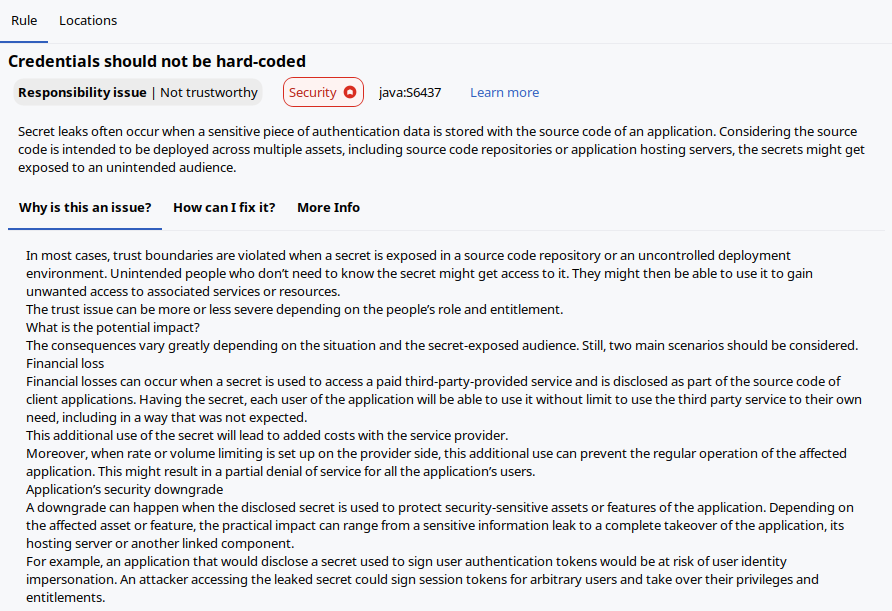
\includegraphics[width=3cm]{images/sonarlint-report.png}};
   \draw[gray,-Kite] ([xshift=6mm]dfg-constraints.south) to[out=-40,in=180] (sonar-com.west);
\end{uncoverenv}
\begin{onlyenv}<18-29|handout:2>
\onslide<18->{
   \pgfinterruptboundingbox
   \fill[white,fill opacity=.85] ([yshift=6mm]current page.south west) rectangle (current page.east|-persp.north);
   \endpgfinterruptboundingbox
   \node[draw=darkgray,fill=white,minimum width=4.2cm,minimum height=4.5cm,fill opacity=.93,rounded corners=3.45pt,thick,align=center,right] (@1) at ([xshift=-5mm,yshift=4mm]@code-file.west) {~\\[-5mm]{\onslide<19->{\usebox\ExampleCodeCfG}}};
   \node[above] at(@1.south) {\textbf{Code}};
}
\onslide<20->{
   \node[draw=darkgray,fill=white,minimum width=4cm,minimum height=4.5cm,fill opacity=.93,rounded corners=3.45pt,thick,right=7mm,align=center] (@2) at (@1.east) {%
   ~\\[-5mm]{\onslide<21->{\resizebox{4cm}!{\usebox\ExampleCFGofCode}}}%
   };
   \node[above] at(@2.south) {\textbf{Control Flow Graph}};
}
\onslide<23->{
   \node[draw=darkgray,fill=white,minimum width=4cm,minimum height=4.5cm,fill opacity=.93,rounded corners=3.45pt,thick,right=7mm,align=center] (@3) at (@2.east) {~\\[-5mm]{\onslide<24->{\resizebox{4cm}!{\usebox\ExampleLivenessofCode}}}};
   \pgfinterruptboundingbox
   \node[xshift=-12mm,yshift=4.2mm,draw=darkgray,fill=white,fill opacity=.93,rounded corners=3.45pt,thick,align=center,text width=4.5cm,scale=.65,font=\footnotesize,inner sep=1pt] at(@3.north east) {%
   \begin{align*}
      \mathbf{In}_n &= (\mathbf{Out}_n - \mathbf{Kill}_n) \cup \mathbf{Gen}_n \\
      \mathbf{Out}_n &= \begin{cases}
         \mathbf{BI} & n \text{~is End} \\
         \bigcup\limits_{m \in \text{succ}(n)} \mathbf{In}_m & \text{otherwise}
      \end{cases}
   \end{align*}
   With fixpoint iteration
   };
   \endpgfinterruptboundingbox
   \node[above] at(@3.south) {\textbf{Liveness}\textsuperscript{\smaller[2]\cite[p.\,26]{10.5555/1592955}}};
}
\end{onlyenv}
% by default iterated until reach fixpoint
\end{tikzpicture}
\end{lrbox}
\global\setbox\SonarLintShow=\copy\SonarLintShow
\begin{tikzpicture}[overlay,remember picture]
   \node[above=-1mm,xshift=.33mm] at(current page.south) {\usebox\SonarLintShow};
\end{tikzpicture}
\end{uncoverenv}
\begin{tikzpicture}[overlay,remember picture]
   \node[below left=4mm] at(current page.north east) {\Logo[2.5cm]{https://www.sonarsource.com/products/sonarlint/}{sonar}};
   \node[above right,yshift=4mm,bottom note] at(current page.south west) {\href{https://github.com/SonarSource}{github.com/SonarSource/sonar-java}};
   \only<23-|handout:2>{
      \node[above left,bottom note,yshift=4mm] at(current page.south east) {\cite{10.5555/1592955}~\citetitle{10.5555/1592955} (\citeauthor{10.5555/1592955})};
   }
\end{tikzpicture}
\end{frame}

\lstfs{11}
\begin{frame}[t,fragile]{\textcolor{gray}{SonarLint ---~}Unused Assignments}
\begin{itemize}
   \itemsep9pt
   \item<2-> Analyze \enquote{Dead Stores} {\onslide<3->{\smaller[2]\textcolor{gray}{(in 311\,loc\,/\,259\,cloc)}:}}
\begin{minted}[escapeinside=||]{java}
|\onslide<4->|int x = 0;
x = 42;|\onslide<1->|
\end{minted}
   \item<5-> Use \href{https://github.com/SonarSource/sonar-java/blob/50b7d48e5764545a78a7ef2bf84b8a5ff1f30b3e/java-frontend/src/main/java/org/sonar/java/cfg/LiveVariables.java\#L73}{liveness analysis} to obtain \(out_n\) of each basic block in the CFG
   \item<6-> Check if assignments (\bjava{x =}, \bjava{x++},~\ldots) are in \(out_n\) and resolved
   \item<7-> Check overwrites in the same basic block
   \item<8-> Minor special handling for \bjava{try-finally} blocks,~\ldots
\end{itemize}
\begin{tikzpicture}[overlay,remember picture]
   \node[below left=4mm] at(current page.north east) {\Logo[2.5cm]{https://www.sonarsource.com/products/sonarlint/}{sonar}};
   \node[above right,bottom note, yshift=4mm] at(current page.south west) {\href{https://github.com/SonarSource/sonar-java/blob/50b7d48e5764545a78a7ef2bf84b8a5ff1f30b3e/java-checks/src/main/java/org/sonar/java/checks/DeadStoreCheck.java\#L52}{Implementation of Rule S1854}};
   \begin{uncoverenv}<9-|handout:2>
      \xlstsetmintedstyle{plain number}
      \node[above left=2mm,yshift=5.5mm,text width=.75\paperwidth,fill=white,draw,rounded corners=3pt,inner ysep=0pt,fill opacity=.95,drop shadow={fill=lightgray!50}] at(current page.south east) {\lstfs{8}%
\begin{minted}[firstnumber=77,morekeywords={[3]{CFG,Block,LiveVariables}},xleftmargin=7mm,prebreak={}]{java}
LiveVariables liveVariables = LiveVariables.analyze(cfg);
// Liveness analysis provides information only for block boundaries, so we should do analysis between elements within blocks
for(CFG.Block block : cfg.blocks()) {
   checkElements(block, liveVariables.getOut(block), methodSymbol);
}
\end{minted}
      };
   \end{uncoverenv}
\end{tikzpicture}
\end{frame}


\begin{frame}[t,fragile]{\textcolor{gray}{SonarLint ---~}Hardcoded Credentials}
\begin{itemize}
   \itemsep8pt
   \item<2-> It does not always have to be that heavy! {\onslide<3->{\smaller[2]\textcolor{gray}{(116\,loc\,/\,87\,cloc may suffice)}}}
   \item<4-> For example, to identify hardcoded credentials:
{%
\lstfs{9}
\begin{minted}[escapeinside=||]{java}
|\onslide<5->|new PasswordAuthentication("password", "secret".toCharArray());|\onslide<1->|
\end{minted}
}\vspace*{-.85\baselineskip}
   \item<6-> Traverse the Abstract Syntax Tree~(AST)
   \item<7-> Check calls against a long \href{https://github.com/SonarSource/sonar-java/blob/3e2cb4478100a5ea082dde30004067579eef58a4/java-checks-aws/src/main/resources/org/sonar/java/checks/security/S6437-methods.json}{list of signatures} (currently 7664) with problematic indices
   \item<8-> Check if the arguments are \enquote{constant}\\
   \onslide<9->{\textcolor{gray}{visiting the dataflow links and checking for predefined \enquote{plain text}}}
\end{itemize}
\begin{tikzpicture}[overlay,remember picture]
   \node[below left=4mm] at(current page.north east) {\Logo[2.5cm]{https://www.sonarsource.com/products/sonarlint/}{sonar}};
   \node[above right,bottom note, yshift=4mm] at(current page.south west) {\href{https://github.com/SonarSource/sonar-java/blob/50b7d48e5764545a78a7ef2bf84b8a5ff1f30b3e/java-checks-aws/src/main/java/org/sonar/java/checks/security/HardCodedCredentialsShouldNotBeUsedCheck.java\#L43}{Implementation of Rule S6437}};
   % TODO: mark heuristics: list of signatures and constant check
   \begin{uncoverenv}<10-|handout:2>
      \xlstsetmintedstyle{plain number}
      \xlstblacklistlinenumbers{111}
      \node[above left=2mm,yshift=5.5mm,text width=.85\paperwidth,fill=white,draw,rounded corners=3pt,inner ysep=0pt,fill opacity=.95,drop shadow={fill=lightgray!50}] at(current page.south east) {\lstfs{8}%
\begin{minted}[firstnumber=107,morekeywords={[3]{ExpressionTree,JavaFileScannerContext,Location,ISSUE_MESSAGE}},xleftmargin=7mm,prebreak={}]{java}
for (int targetArgumentIndex : method.indices) {
   ExpressionTree argument = arguments.get(targetArgumentIndex);
   var secondaryLocations = new ArrayList<JavaFileScannerContext.Location>();
   if (isExpressionDerivedFromPlainText(argument, 
               secondaryLocations, new HashSet<>())) {
      reportIssue(argument, ISSUE_MESSAGE, secondaryLocations, null);
   }
}
\end{minted}
      };
   \end{uncoverenv}
\end{tikzpicture}
\end{frame}

\newsavebox\pinguLook
\savebox\pinguLook{\scalebox{.65}{\tikz{\pingu[left eye wink,right wing wave,magnifier right,small,tie,deer hat]}}} 

\subsubsection{LiSA}
\againframe<7,18|handout:4>{tool-slide}
\begin{frame}{LiSA}
\begin{itemize}
   \itemsep6.5pt
   \item<2-> \textcolor{gray}{(Largely)} Language Independent \underline{Li}brary for \underline{S}tatic \tikzmarknode{lisa-alts}{\underline{A}nalysis}
   \item<4-> Custom frontends for Rust, Go, Python, EVM,~\ldots
\end{itemize}
\begin{tikzpicture}[overlay,remember picture]
   \node[below left=4mm] at(current page.north east) {\Logo[2cm]{https://github.com/lisa-analyzer/lisa}{lisa}};
   \node[above right,yshift=4mm,bottom note] at(current page.south west) {\href{https://github.com/lisa-analyzer/lisa}{github.com/lisa-analyzer/lisa}};
   \onslide<3->{%
      \draw[-Kite,gray] ([xshift=1.5mm]lisa-alts.east) to[out=0,in=180] ++(6mm,2mm) node[right,bottom note,align=left] {Similar to \href{https://mopsa.lip6.fr/}{Mopsa} or \href{https://github.com/antoinemine/apron}{Apron}};
   }
\end{tikzpicture}
\begin{uncoverenv}<5->
\begin{tikzpicture}[o/.style={outer sep=0pt,inner sep=0pt},remember picture]
   \node[o] (@) at (0,0) {\usebox\CodeFile};
   \node[above=2.5mm,xshift=1.15mm,gray] at(@.north) {\textbf{\normalsize Input}};
\pgfonlayer{background}
\scope[transparency group,opacity=.4]
\node[o,rotate around={-30:(@.south east)},anchor=south east] at(@.south east) {\usebox\CodeFile};
\node[o,rotate around={-12:(@.south east)},anchor=south east] at(@.south east) {\usebox\CodeFile};
\endscope
\endpgfonlayer
\coordinate (@) at(@.east);
\foreach[count=\i] \usecase/\targeti in {{\raisebox{1pt}{Textual}}/1,Syntactical/0, Semantical/0, Historical/1, Annotated/0, {\raisebox{-3pt}{Metadata,~\ldots}}/1} { % program spectra, hardware, contexts, ...
\pgfmathsetmacro\rot{-24*\i+66}
      \path ([xshift=.5mm]@.east)++(\rot+10:1mm) coordinate (@a);
      \fill[opacity=.18,gray] (@a.east) -- ++(\rot:1.5cm) arc (\rot:\rot+20:1.5cm) -- cycle;
      \draw[thick,gray] (@a.east)++(\rot:1.5cm) arc (\rot:\rot+20:1.5cm);
      \tikzset{@/.style={}}
      \ifnum\targeti=1relax
         \only<7->{
            \tikzset{@/.style={opacity=.2}}
         }
      \fi
      \path (@a.east) -- ++(1.05*\rot+10:1.6cm) node[right,font=\small,darkgray,@] (@uc-\i) {\vphantom{a}\smash{\usecase}};
}
\coordinate (@east) at (current bounding box.east);
\onslide<8->{%
   \draw[decoration={brace},decorate,gray] ([yshift=.5mm]@uc-2.north east-|@uc-3.north east) -- ([yshift=-.5mm]@uc-3.south east) node[midway,right=1mm,font=\footnotesize,align=left] (jbc) {Construct CFG}; % using java byte code is rather common
}
\node[above=1.65mm,xshift=1mm,gray] at(current bounding box.north) {\textbf{\normalsize Perspectives}};
\begin{onlyenv}<-5|handout:0>
\node[right,yshift=-7mm,xshift=1cm,align=left,font=\small,darkgray,text width=3.25cm] (@techn) at(@east){{{{Text/Code Search}\strut}}~\\[4mm]\strut{{{Clustering}}}~\\[4mm]\strut{{{Abstract Domains}}}~\\[4mm]\strut{{{Dataflow Constraints}}}~\\[1mm]\strut{{\centerline{\footnotesize\(\vdots\)}}}};
\node[above=1.5mm,gray,xshift=-4.5mm] at(@techn.north) {\textbf{\normalsize Theory}};
\scope[gray,line cap=round]
   \draw ([yshift=1.5pt]@uc-1.east) -- ([yshift=-2.5mm]@techn.north west);
   \draw ([yshift=1.5pt]@uc-2.east) -- ([yshift=-2.5mm]@techn.north west);
   \draw[densely dotted] ([yshift=1.5pt]@uc-3.east) -- ([yshift=-2.5mm]@techn.north west);
   \draw ([yshift=1.5pt]@uc-1.east) -- ([yshift=-10.5mm]@techn.north west);
   \draw ([yshift=0pt]@uc-2.east) -- ([yshift=-10.5mm]@techn.north west);
   \draw ([yshift=1.5pt]@uc-4.east) -- ([yshift=-10.5mm]@techn.north west);
   
   \draw ([yshift=-1pt]@uc-2.east) -- ([yshift=-18.5mm]@techn.north west);
   \draw ([yshift=-1pt]@uc-3.east) -- ([yshift=-18.5mm]@techn.north west);
   \draw ([yshift=1.5pt]@uc-5.east) -- ([yshift=-18.5mm]@techn.north west);
   
   \draw ([yshift=-1pt]@uc-2.east) -- ([yshift=-26mm]@techn.north west);
   \draw ([yshift=-1pt]@uc-3.east) -- ([yshift=-26mm]@techn.north west);
\endscope
   
   \node[right=7.5mm] (@) at(current bounding box.east) {\resizebox*!{2.85cm}{\usebox\UiBox}};
   \scope[transparency group,opacity=.5,every path/.append style={line cap=round,line width=.5pt}]
      \draw[-Kite,gray] ([yshift=-2.5mm,xshift=-6.5mm]@techn.north east) to[out=0,in=180] ([xshift=1.5mm,yshift=-6.35mm]@.west);
      \draw[-Kite,gray] ([yshift=-10.5mm,xshift=-18.5mm]@techn.north east) to[out=0,in=180] ([xshift=7.15mm,yshift=-1.35mm]@.west);
      \draw[-Kite,gray] ([yshift=-18.5mm,xshift=-6.25mm]@techn.north east) to[out=0,in=180] ([xshift=26.15mm,yshift=-9.35mm]@.west);
      \draw[-Kite,gray] ([yshift=-26mm,xshift=-2.5mm]@techn.north east) to[out=0,in=180] ([xshift=26.15mm,yshift=-9.35mm]@.west);
   \endscope
   \node[above, gray] at(@.north) {\tiny \textbf{\normalsize Communicate} or \textbf{\normalsize Use}};
\end{onlyenv}
\onslide<9->{%
   \draw[gray,-Kite] (@uc-5.east) to[out=0,in=180] ++(6.5mm,2mm) node[below right,font=\footnotesize,yshift=.7\baselineskip,align=left] {(Depends on Frontend)};
}
\onslide<10->{%
   \draw[gray,Kite-] (jbc) to[out=80,in=260] ++(2mm,7.5mm) node[above,bottom note,align=center] {Language-Specific\\Frontends};
}
\onslide<11->{%
   \draw[gray,-Kite] ([xshift=-4.25mm]jbc.south) to[out=-80,in=180] ++(6mm,-3mm) node[right,bottom note,align=center] (cfg-dr-note) {\href{https://github.com/lisa-analyzer/lisa/blob/2543b47cfdb0a968a064d16f000fa0ad1d823125/lisa/lisa-analyses/src/main/java/it/unive/lisa/analysis/dataflow/Liveness.java\#L25}{Liveness}, \href{https://github.com/lisa-analyzer/lisa/blob/cd351110a5c47f69a16f0ca025058ad5a53976cb/lisa/lisa-analyses/src/main/java/it/unive/lisa/analysis/numeric/Pentagon.java\#L47}{Pentagons},~\ldots};
}
\onslide<12->{
   \node[above=3.5mm,gray,xshift=20.5mm] (theory) at(@techn.north) {\textbf{\normalsize Theory}};
}
\onslide<13->{
   \node[below=1mm,align=right] (a-domains) at(theory.south) {\small Abstract Domains}; % many parameterized
}
\onslide<14->{
   \draw[gray,Kite-Kite] (a-domains.south) to[bend left] (cfg-dr-note.east);
}
\begin{uncoverenv}<15->
   \node[right=20.5mm,yshift=-.5mm,gray] (communicate) at(theory.east) {\textbf{\normalsize Use}};
   \node[below=1mm,thick,inner sep=0pt,align=center,font=\small] (lisa-use) at(communicate.south) {Extension Interfaces\\Fixpoint Iterations,\\\ldots};
   \draw[gray,-Kite] ([xshift=1mm]a-domains.south) to[out=-40,in=180] (lisa-use.west);
\end{uncoverenv}
\onslide<16->{%
   \node[above left=2mm,yshift=3mm] (@ping) at(current page.south east) {\usebox\pinguLook};
   \node[left,gray,align=right] at(@ping.west) {Let's have a\\closer look!};
}
\end{tikzpicture}
\end{uncoverenv}
\end{frame}

\begin{lrbox}{\IntervalLattice}
\scriptsize
\begin{tikzpicture}[line cap=round,x=6.5mm,y=6.5mm,gray]
   \matrix (A) [matrix of nodes, row sep=2.5mm, column sep=-2mm]
   {
       & &  & \I{-1}{\infty} & & & \\
       & & \I{-1}{1} & \ldots & \I{0}{2} & & \\
      & \I{-1}{0} & \ldots & \I01 & \ldots & \I{1}{2} & \\
      \I{-1}{-1} & \ldots & \I00 & \ldots & \I11 & \ldots & \I22 \\
      & & & \absexpr{\bot} & & & \\
   };
   \scope[line cap=round]
   \draw (A-2-3) -- (A-3-2) -- (A-4-1) -- (A-5-4);
   \draw (A-3-6) -- (A-4-7) -- (A-5-4);
   \draw (A-3-2) -- (A-4-3) -- (A-3-4) (A-3-4) -- (A-4-5) -- (A-3-6);
   \draw (A-2-3) -- (A-3-4) (A-3-4) -- (A-2-5) -- (A-3-6);
   \draw (A-4-3) -- (A-5-4) -- (A-4-5);
   \draw[densely dotted] (A-2-5) -- (A-1-4) -- (A-2-3);
   \draw[densely dotted] (A-5-4) -- ++(-1,0.05)  (A-5-4) -- ++(1,0.05);
   \foreach[count=\y] \i in {4,3,2,1} {
      \draw[densely dotted] (A-\y-\i.north west) -- ++(-.4,0.14);
      \node[left=3.5mm] at(A-\y-\i.west) {\footnotesize\ldots};
      \pgfmathsetmacro\other{int(8-\i)}
      \draw[densely dotted] (A-\y-\other.north east) -- ++(.4,0.14);
      \node[right=3.5mm] at(A-\y-\other.east) {\footnotesize\ldots};
   }
   \node[above=3.5mm] (pz) at(A-1-4.north) {\absexpr{\top}};
   \draw[densely dotted] (pz) -- ++(-1.25,-0.1) (pz) -- ++(1.25,-0.1);
   \endscope
\end{tikzpicture}
\end{lrbox}

\makeatletter
% https://github.com/lisa-analyzer/lisa/blob/bd00779ab87e1cd31ed01b97d9b0e71b922f5bcf/lisa/lisa-analyses/src/main/java/it/unive/lisa/analysis/numeric/Interval.java#L47
\def\FakeLineNumber#1{\llap{\xlstGetStyle{linenumbers}\href{https://github.com/lisa-analyzer/lisa/blob/bd00779ab87e1cd31ed01b97d9b0e71b922f5bcf/lisa/lisa-analyses/src/main/java/it/unive/lisa/analysis/numeric/Interval.java\#L#1}{\underline{\xlst@lst@num@consume{#1}}}~~~}}

\begin{frame}[fragile]{\textcolor{gray}{LiSA ---~}Interval Analysis\textsuperscript{\color{gray}\smaller[2]\cite[p.\,389]{cousout2021principles}}}
\lstfs{8}
\begin{uncoverenv}<7->
{\scriptsize\color{gray}\href{https://github.com/lisa-analyzer/lisa/blob/bd00779ab87e1cd31ed01b97d9b0e71b922f5bcf/lisa/lisa-analyses/src/main/java/it/unive/lisa/analysis/numeric/Interval.java}{\hbox{\faFileCodeO~}lisa-analyses/src/main/java/it/unive/lisa/analysis/numeric/Interval.java} (simplified)}
\AnimateCode{onslide={o1:{2},-,o3:{4,...,7},o8:{9,...,13},-,0,-},first slide=7,handout=12/1}
\begin{minted}[morekeywords={Interval,IntInterval,Constant,ProgramPoint,SemanticOracle,SemanticException},escapeinside=||]{java}
|\FakeLineNumber{57}|Interval TOP = new Interval(IntInterval.INFINITY);
|\onslide<8->{\FakeLineNumber{62}}\onslide<8->|Interval BOTTOM = new Interval(null);|\medskip|
|\onslide<9->{\FakeLineNumber{273}}\onslide<9->|public Interval lubAux(Interval other) {
|\onslide<9->{\FakeLineNumber{276}}\onslide<9->|   var newL = getLow().min(other.getLow());
|\onslide<9->{\FakeLineNumber{277}}\onslide<9->|   var newH = getHigh().max(other.getHigh());
|\onslide<9->{\FakeLineNumber{278}}\onslide<9->|   return new Interval(newLow, newHigh);
|\onslide<9->{\FakeLineNumber{279}}\onslide<9->|}|\medskip\onslide<1->|
|\onslide<10->{\FakeLineNumber{282}}\onslide<10->|public Interval glbAux(Interval other) {
|\onslide<10->{\FakeLineNumber{284}}\onslide<10->|   var newL = getLow().max(other.getLow());
|\onslide<10->{\FakeLineNumber{285}}\onslide<10->|   var newH = getHigh().min(other.getHigh());|\onslide<1->|
|\onslide<10->{\FakeLineNumber{287}}\onslide<11->|   if(newLow.compareTo(newHigh) > 0) return bottom();
|\onslide<11->{\FakeLineNumber{289}}\onslide<10->|   return new Interval(newLow, newHigh);
|\onslide<10->{\FakeLineNumber{290}}\onslide<10->|}|\vspace*{-5mm}\onslide<1->|
\end{minted}
\endAnimateCode
\onslide<12->{\footnotesize\textit{Widening, Narrowing, Assume, Satisfies,~\ldots}}
\end{uncoverenv}
\begin{tikzpicture}[overlay,remember picture]
   \node[above right,yshift=4mm,bottom note] at(current page.south west) {\cite{cousout2021principles}~\citetitle{cousout2021principles} (\citeauthor{cousout2021principles})};
   \onslide<2->{\node[above left,yshift=5mm,scale=.8] (int-latt) at(current page.south east) {\usebox\IntervalLattice};}
   \onslide<3->{%
      \node[above,text width=5cm,font=\scriptsize] at(int-latt.north) {%
         \begin{align*}
            \top &= \I{-\infty}{\infty} \tag*{Top}\\
            \onslide<4->{\bot} &\onslide<4->{{}= \absexpr{\emptyset} \only<4->{\tag*{Bottom}}} \\
            \onslide<5->{\absexpr{\Lub_{k}} \I{\ell_k}{h_k}} &\onslide<5->{{}=\I{\min(\ell_k)}{\max(h_k)} \only<5->{\tag*{Join}}} \\
            \onslide<6->{\absexpr{\Glb_{k}} \I{\ell_k}{h_k}} &\onslide<6->{{}=\I{\max(\ell_k)}{\min(h_k)} \only<6->{\tag*{Meet}}}
            % hidden for now
            % \I{\ell_l}{h_l} \absexpr{\widen} \I{\ell_r}{h_r} &= \I{\ell_l > \ell_r ? -\infty : \ell_l}{h_l < h_r ? \infty : h_l} \tag*{Widening}
         \end{align*}
      };
   }
\end{tikzpicture}
\end{frame}

\begin{frame}[fragile]{\textcolor{gray}{LiSA ---~}Interval Analysis\textsuperscript{\color{gray}\smaller[2]\cite[p.\,389]{cousout2021principles}}\hfill Semantics}
\lstfs{8}
\onslide<2->{When to create which interval?}\\*
\begin{uncoverenv}<3->
{\scriptsize\color{gray}\href{https://github.com/lisa-analyzer/lisa/blob/bd00779ab87e1cd31ed01b97d9b0e71b922f5bcf/lisa/lisa-analyses/src/main/java/it/unive/lisa/analysis/numeric/Interval.java}{\hbox{\faFileCodeO~}lisa-analyses/src/main/java/it/unive/lisa/analysis/numeric/Interval.java} (simplified)}
\AnimateCode{onslide={o1:{3,...,8},-,-,o9:{10},o11:{12},o1:{3,...,12},-},first slide=3,handout=8/1}
\preto\ldots{\color{lightgray}}% hijack the literate
\begin{minted}[morekeywords={Interval,IntInterval,Constant,ProgramPoint,SemanticOracle,SemanticException},escapeinside=||]{java}
|\onslide<3->{\FakeLineNumber{144}}\onslide<3->|public Interval evalNonNullConstant(Constant constant,
|\onslide<3->{\FakeLineNumber{146}}\onslide<3->|      ProgramPoint pp, SemanticOracle oracle) {
|\onslide<4->{\FakeLineNumber{148}}\onslide<4->|   if(constant.getValue() instanceof Integer) {
|\onslide<4->{\FakeLineNumber{149}}\onslide<4->|      var i = (Integer) constant.getValue();
|\onslide<4->{\FakeLineNumber{150}}\onslide<4->|      return new Interval(i, i);
|\onslide<4->{\FakeLineNumber{151}}\onslide<4->|   }
|\onslide<5->{\FakeLineNumber{152}}\onslide<5->|   return top();|\onslide<1->|
|\onslide<3->{\FakeLineNumber{153}}\onslide<3->|}|\medskip\onslide<1->|
|\onslide<6->{\FakeLineNumber{157}}\onslide<6->|public Interval evalUnaryExpression(UnaryOperator op,
|\onslide<6->{\FakeLineNumber{158}}|    Interval arg, :ldots:) { :ldots: }|\onslide<1->|
|\onslide<7->{\FakeLineNumber{188}}\onslide<7->|public Interval evalBinaryExpression(BinaryOperator op,
|\onslide<7->{\FakeLineNumber{189}}|    Interval left, |\tikzmarknode{fold-like-marker}{\strut}|Interval right, :ldots:) { :ldots: }|\onslide<1->|
\end{minted}
\endAnimateCode
\end{uncoverenv}
\begin{tikzpicture}[overlay,remember picture]
   \node[above right,yshift=4mm,bottom note] at(current page.south west) {\cite{cousout2021principles}~\citetitle{cousout2021principles} (\citeauthor{cousout2021principles})};
   \node[above left,yshift=5mm,scale=.8] (int-latt) at(current page.south east) {\usebox\IntervalLattice};
   \onslide<9->{%
      \coordinate (@) at(fold-like-marker);
      \draw[Kite-,gray] ([xshift=5mm,yshift=-1mm]@) to[out=280,in=180] ++(3mm,-4mm) node[right,bottom note] {Fold-like Evaluation};
   }
\end{tikzpicture}
\end{frame}

\subsubsection{flowR}
\let\T\texttt
\def\Content#1#2{#1\\[-.6ex]\smaller\textit{\color{gray}#2}}
\againframe<7,21|handout:7>{tool-slide}
\newsavebox\ShookPingu
\savebox\ShookPingu{\tikz{\pingu[wings shock,eyes shock,tie]}}

\newsavebox\PartyPingu

\savebox\PartyPingu{\tikz{\pingu[wings wave,eyes wink,tie=purple]}}
\begin{frame}[fragile]{flowR}
   \lstfs{8}
   \begin{itemize}
      \itemsep6pt
      \item<2-> A static analysis framework for R
      \item<3-> Developed here, at Ulm University \onslide<4->{\smash{\raisebox{-4pt}{\resizebox*!{1.5\baselineskip}{\usebox\PartyPingu}}}}\\*[1mm]
         \onslide<5->{\color{gray}{\only<6->{\bfseries\color{black}}Florian Sihler}, \color{gray}Julian Schubert, Lars Pfrenger, Johanna Scheck, Lukas Pietzschmann,\\Ruben Dunkel, Felix Schlegel, Pascal Deusch,~\ldots}%
      \item<7-> Let's get back to R:
\begin{uncoverenv}<8->
   \begin{columns}[onlytextwidth,c]
\column{.04\linewidth}
\column{.3\linewidth}
\begin{minted}{R}
x <- 4
f <- function() x
body(f) <- quote(y)
y <- 42
f() # 42
\end{minted}
\column{.365\linewidth}
\color{black}\vspace*{-\baselineskip}%
\begin{minted}{R}
`if` <- function(...) 42
if(TRUE) print(3) # 42
\end{minted}
\column{.3\linewidth}
\color{black}\vspace*{-\baselineskip}%
\begin{minted}{R}
x <- 2
`<-` <- `*`
x <- 21 # 42
\end{minted}
\end{columns}
\end{uncoverenv}
\item<9-> We have to intertwine dataflow- and control-flow analysis\ldots
\end{itemize}
   \begin{tikzpicture}[overlay,remember picture]
      \node[below left=4mm,yshift=2mm] at(current page.north east) {\Logo[2.1cm]{https://github.com/flowr-analysis/flowr}{flowr}};
      \node[above right,yshift=4mm,bottom note] at(current page.south west) {\href{https://github.com/flowr-analysis/flowr}{github.com/flowr-analysis/flowr}};
   \end{tikzpicture}
\end{frame}

\def\SwitchTo#1#2{#1}
\def\GrayBack{\fill[white,opacity=.7] (current bounding box.south west) rectangle (current bounding box.north east);}
\def\XShift{3.5mm}%
\newsavebox\CodeBoxA
% \begin{frame}[fragile,c]{\textcolor{gray}{flowR ---} Architecture}
% \centering
% \begin{tikzpicture}[All Soft, br/.style={fill=white,draw=black,drop shadow={fill=lightgray!50},minimum width=2.5cm,minimum height=1.5cm,signal,signal from=west,signal to=east,signal pointer angle=125,rounded corners=2pt},k/.style={below,font=\footnotesize,xshift=-.33mm,color=darkgray},m/.style={above,font=\scriptsize,xshift=-.33mm,color=gray},BaseGray,Link/.style={
%    draw=SoftGray,
%    line width=1.5pt,
%    line cap=round,
%    line join=round,
%    -%
% }]
%    \tikzset{a/.style={opacity=.5}}
%    \coordinate (@) at (0,0);

%    \onslide<2->{
%       \node[br,right=\XShift] (@) at (@.east) {};
%       \coordinate (@parse) at (@.north west);
%       \coordinate (@parse-l) at (@.south west);
%       \node (r-conv) at (@) {\SwitchTo{\usebox\Parsing}{\,Parse}};
%       \pgfinterruptboundingbox\node[k] at (@.south) {\SwitchTo{Parse}{}};\endpgfinterruptboundingbox
%    }
%       % \onslide<4->{\node[m] at (@.north) {\texttt{parse}\,\(\to\)\,XML};}

%    \onslide<3->{
%       \node[br,right=\XShift] (@) at (@.east) {};
%       \node[align=center] (first-ast) at (@) {\SwitchTo{\usebox\FirstAst}{Normalize}};
%       \coordinate (@normalize) at (@.north west);
%       \pgfinterruptboundingbox\node[k,align=center] at (@.south) {\SwitchTo{Normalize}{}};\endpgfinterruptboundingbox
%       % \onslide<6->{\node[m] at (@.north) {in TypeScript};}
%       \coordinate (@l) at(@.south west);
%    }
%    \scope
%    \onslide<4->{
%       \node[br,right=\XShift] (@) at (@.east) {};
%       \coordinate (@dataflow) at (@.north east);
%       \coordinate (@dataflow-l) at (@.south east);
%       \node (dataflow) at (@) {\SwitchTo{\usebox\DataFlow}{\;Dataflow}};
%       \pgfinterruptboundingbox\node[k] at (@.south) {\SwitchTo{Dataflow}{}};\endpgfinterruptboundingbox
%    }
%    \endscope
%    \scope
%    \onslide<5->{
%       \node[br,right=\XShift] (@) at (@.east) {};
%       \pgfinterruptboundingbox\node (slicing) at (@) {\SwitchTo{\usebox\Slicing}{\,Slice}};\endpgfinterruptboundingbox
%       \node[k] at (@.south) {\SwitchTo{Slice}{}};
%       \coordinate (@slice) at (@.north west);
%       \coordinate (@slice-l) at (@.south west);
%       % \onslide<9->{\node[m] at (@.north) {Weiser~\cite{weiser_program_1984}};}
%    }
%    \endscope
%    \onslide<6->{
%       \node[br,right=\XShift] (@) at (@.east) {};
%       \node (reconstruct) at (@) {\SwitchTo{\usebox\Reconstruct}{\; Reconstruct}};
%       \pgfinterruptboundingbox\node[k] at (@.south) {\SwitchTo{Reconstruct}{}};\endpgfinterruptboundingbox
%       \coordinate (@r) at(@.south east);
%       \coordinate (@reconstruct) at (@.north east);
%       \coordinate (@reconstruct-l) at (@.south east);
%    }
% \end{tikzpicture}\medskip
% \begin{onlyenv}<7->
% \lstfs{7}
% \hspace*{1.5cm}%
% \begin{lrbox}\CodeBoxA
% \begin{minted}[deletekeywords={sum,prod},escapeinside={/*}{*/}]{R}
% sum  <- 0
% prod <- 1
% n    <- 10

% for (i in 1:(n-1)) {
%    sum  <- sum + i
%    prod <- prod * i
% }

% cat("Sum:"/*\color{black}*/, /*\texttt{\only<8->{\textbf}{sum}}*//*\color{black}*/, "\n")
% cat/*\color{black}*/("Product:"/*\color{black}*/, prod, "\n"/*\color{black}*/)
% \end{minted}
% \end{lrbox}
% \begin{tikzpicture}
% \begin{uncoverenv}<7->
% \node (@) at (0,0) {%
%    \usebox\CodeBoxA
% };
% \end{uncoverenv}

% \begin{uncoverenv}<9->
%    \node[right=2.5cm] (@2) at (@.east) {%
% \AnimateCode{onslide={o8:{7,5,4,3,1}}, first slide=9,handout={9/1}}
% \begin{minted}[deletekeywords={sum,prod},escapeinside={/*}{*/}]{R}
% sum  <- 0
% prod <- 1
% n    <- 10

% for (i in 1:(n-1)) {
%    sum  <- sum + i
%    prod <- prod * i
% }

% cat("Sum:", sum, "\n")
% cat("Product:", prod, "\n")
% \end{minted}
% \endAnimateCode
%    };
% \end{uncoverenv}
% \onslide<8->{
%    \draw[-Kite,line cap=round] ([xshift=5mm]@.east) to[edge node={node[above] {\footnotesize\texttt{slice({\xlstGet{linenumbers}{\footnotesize10}}\footnotesize\color{black}, \textbf{sum})}}}] ([xshift=-5mm]@2.west);
% }
% \end{tikzpicture}\hspace*{-2cm}
% \end{onlyenv}
% \begin{tikzpicture}[overlay,remember picture]
%    \node[below left=4mm,yshift=2mm] at(current page.north east) {\Logo[2.1cm]{https://github.com/flowr-analysis/flowr}{flowr}};
%    \node[above right,yshift=4mm,bottom note] at(current page.south west) {\href{https://github.com/flowr-analysis/flowr/tree/main/src/dataflow}{github.com/flowr-analysis/flowr/tree/main/src/dataflow}};
% \end{tikzpicture}
% \end{frame}






\lstfs{8}
\tikzset{K/.style={midway,#1=-.5mm,font=\smaller[3]}}
\newsavebox\FinalDataFlow
\colorlet{lgray}{gray!50!white}
\def\MarkBox#1{#1}%TODO: \fcolorbox{lgray}{white}{#1}}
\newcommand\MarkAt[3][0]{\setbox0=\hbox{~#3~}\makebox[\wd0+1mm][c]{\null\hfill\only<#2|handout:#1>{\bfseries\fboxsep=1pt\expandafter\larger\MarkBox}{\smash{#3}}\null\hfill}}
\newsavebox\EmptyEnvBox
\tikzset{%
   Env/.style={text width=1.85cm,rounded corners=2pt,fill=white,font=\footnotesize},
}%
\def\GetWith#1{\tikz{%
\node[Env] (@) {\strut#1};
\pgfonlayer{background}
\fill[rounded corners=2pt,fill=lgray] ([shift={(.4mm,.4mm)}]@.north east) rectangle ([shift={(-.4mm,-.4mm)}]@.south west);
\pgfinterruptboundingbox
\node[above right,gray] at([xshift=-1mm]@.north west) {\scriptsize Environment};
\endpgfinterruptboundingbox
\endpgfonlayer
}}
\newsavebox\EnvBox
\setbox\EnvBox=\hbox{}
\savebox\EmptyEnvBox{\GetWith{}}
\def\mto#1{\kern1.5pt$\mapsto$\kern1.5pt\bIndexR{#1}}
\newsavebox\BoxWithX \savebox\BoxWithX{\GetWith{x\mto{x_0}}}
\newsavebox\BoxWithXY \savebox\BoxWithXY{\GetWith{x\mto{x_0},\,y\mto{y_0}}}
\newsavebox\BoxWithZ \savebox\BoxWithZ{\GetWith{z\mto{z_0}}}
\newsavebox\BoxWithFull \savebox\BoxWithFull{\GetWith{x\mto{x_0},\,y\mto{y_0},\,\allowbreak z\mto{z_0}}}
\newcommand<>\OpaOn[1]{\tikzset{@@/.style={}}\only#2{\tikzset{@@/.style={opacity=.4}}}\scope[transparency group,@@]#1\endscope}

\tikzset{
   comm/.style={rectangle,draw=gray,text width=9mm,align=center,minimum height=5mm,font=\ttfamily,fill=white,fill opacity=1,drop shadow={fill=lightgray!50}},
   d/.style={comm,rounded corners=2pt},
   u/.style={comm,rounded rectangle},
   T/.style={font=\scriptsize,gray}
}
\def\WithGraph#1{\tikz{%
#1
\pgfinterruptboundingbox
\node[above=-1.25mm,gray] at(@.north) {\scriptsize\strut Graph};
\endpgfinterruptboundingbox
}}

\iffalse

\newsavebox\XUseGraph \savebox\XUseGraph{\WithGraph{\node[u] (@) at (0,0) {x\textsubscript{0}};}}
\newsavebox\XDefGraph \savebox\XDefGraph{\WithGraph{\node[d] (@) at (0,0) {x\textsubscript{0}};}}
\newsavebox\YUseGraph \savebox\YUseGraph{\WithGraph{\node[u] (@) at (0,0) {y\textsubscript{0}};}}
\newsavebox\ZUseGraph \savebox\ZUseGraph{\WithGraph{\node[u] (@) at (0,0) {z\textsubscript{0}};}}
\newsavebox\YDefGraph \savebox\YDefGraph{\WithGraph{\node[d] (@) at (0,0) {y\textsubscript{0}};}}
\newsavebox\XBUseGraph \savebox\XBUseGraph{\WithGraph{\node[u] (@) at (0,0) {x\textsubscript{1}};}}
\newsavebox\YBUseGraph \savebox\YBUseGraph{\WithGraph{\node[u] (@) at (0,0) {y\textsubscript{1}};}}
\newsavebox\XYBUseGraph \savebox\XYBUseGraph{\WithGraph{\node[u] (@) at (0,0) {y\textsubscript{1}}; \node[u,below=2mm] at (@.south) {x\textsubscript{1}};}}
\newsavebox\XYYBUseGraph \savebox\XYYBUseGraph{\WithGraph{%
   \node[u] (y) at (0,0) {y\textsubscript{1}};
   \node[u,below=2mm] (x) at (y.south) {x\textsubscript{1}};
   \node[d,left=4mm] (z) at (current bounding box.west) {z\textsubscript{0}};
   \draw[-Kite] (z) -- (x);
   \draw[-Kite] (z) -- (y);
   \coordinate(@) at(current bounding box.north);
}}
\newsavebox\FullUseGraph \savebox\FullUseGraph{\WithGraph{%
   \node[u] (y) at (0,0) {y\textsubscript{1}};
   \node[u,below=2mm] (x) at (y.south) {x\textsubscript{1}};
   \node[d,left=4mm] (z) at (current bounding box.west) {z\textsubscript{0}};
   \node[d,right=4mm] (xb) at(x.east) {x\textsubscript{0}};
   \node[d,right=4mm] (yb) at(y.east) {y\textsubscript{0}};
   \draw[-Kite] (z) -- (x);
   \draw[-Kite] (z) -- (y);
   \draw[densely dotted,-Kite] (x) -- (xb);
   \draw[densely dotted,-Kite] (y) -- (yb);
   \coordinate(@) at(current bounding box.north);
}}

\begin{frame}[fragile]{\textcolor{gray}{flowr ---} Dataflow}
% TODO: complete from 2.17 with read-graphs propagation
\hypertarget<1>{@DataFlow}{}%
\lstfs{8}
\begin{minted}[escapeinside={/*}{*/},lineskip=4pt]{IndexR}
/*\onslide<2->*/x_0 <- 21
y_0 <- 2
z_0 <- x_1 * y_1/*\onslide<1->*/
\end{minted}
\begin{center}
\begin{onlyenv}<3|handout:0>
\begin{forest}
   T, for tree={l sep=2mm,s sep=5mm,font=\footnotesize}
   [exprlist, s sep=2cm, l sep=0mm
      [\Content{assignment}{\LeftArrow}, edge label={node[K=above,sloped] {1}}
         [\Content{symbol}{x}, edge label={node[K=above,sloped] {target}}]
         [\Content{number}{21}, edge label={node[K=above,sloped] {source}}]
      ]
      [\Content{assignment}{\LeftArrow}, edge label={node[K=right] {2}},before computing xy={s/.average={s}{siblings}},
         [\Content{symbol}{y}, edge label={node[K=above,sloped] {target}}]
         [\Content{number}{2}, edge label={node[K=above,sloped] {source}}]
      ]
      [\Content{assignment}{\LeftArrow}, edge label={node[K=above,sloped] {3}}
         [\Content{symbol}{z}, edge label={node[K=above,sloped] {target}}]
         [\Content{binary-op}{\raisebox{-5pt}{\large*}}\vspace*{-3mm}, edge label={node[K=above,sloped] {source}},
            [\Content{symbol}{x}, edge label={node[K=above,sloped] {lhs}}]
            [\Content{symbol}{y}, edge label={node[K=above,sloped] {rhs}}]
         ]
      ]
   ]
\end{forest}
\end{onlyenv}
\begin{onlyenv}<4-|handout:1>
\begin{lrbox}\FinalDataFlow
\begin{forest}
   T, for tree={l sep=2mm,s sep=1.5cm, s sep-=5mm,font=\footnotesize}
   [\MarkAt{5,6,21}{exprlist}, s sep=2cm, l sep=0mm,name=exprlist
      [\MarkAt{7,11}{\LeftArrow}, edge label={node[K=above,sloped] {1}},name=la1
         [\MarkAt{8,9}{x\RCodeIndex0}, edge label={node[K=above,sloped] {target}},name=x1]
         [\MarkAt{10}{21}, edge label={node[K=above,sloped] {source}},name=21]
      ]
      [\MarkAt{12,13}{\LeftArrow}, edge label={node[K=right] {2}},name=la2,before computing xy={s/.average={s}{siblings}}
         [y\RCodeIndex0, edge label={node[K=above,sloped] {target}},name=y1]
         [2, edge label={node[K=above,sloped] {source}},name=2]
      ]
      [\MarkAt{14,20}{\LeftArrow}, edge label={node[K=above,sloped] {3}},name=la3
         [\MarkAt{15}{z\RCodeIndex0}, edge label={node[K=above,sloped] {target}},name=z1]
         [\MarkAt{16,19}{\raisebox{-5pt}{\large*}}\vspace*{-3mm}, edge label={node[K=above,sloped] {source}}, name=star,
            [\MarkAt{17}{x\RCodeIndex1}, edge label={node[K=above,sloped] {lhs}},name=x2]
            [\MarkAt{18}{y\RCodeIndex1}, edge label={node[K=above,sloped] {rhs}},name=y2]
         ]
      ]
   ]
\pgfinterruptboundingbox
   \onslide<6-20|handout:0>{\OpaOn<7->{\node[above,scale=.65] at(exprlist.north) {\usebox\EmptyEnvBox};}}
   \onslide<7-10|handout:0>{\OpaOn<8->{\node[above left=-1mm,yshift=-1mm,scale=.65] at(la1.north west) {\usebox\EmptyEnvBox};}}
   % \onslide<8|handout:0>{\node[left,yshift=.5mm,scale=.65] at(x1.west) {\usebox\EmptyEnvBox};}
   \onslide<8->{\OpaOn<9->{\node[left,yshift=.5mm,scale=.65] (@x) at(x1.west) {\usebox\EmptyEnvBox};}}
   \onslide<9->{\OpaOn<10->{\node[below=1mm,scale=.65] at(x1.south) {\usebox\XUseGraph};}}
   \onslide<10->{\OpaOn<11->{\node[below,scale=.65] at(21.south) {\usebox\EmptyEnvBox};}}
   \onslide<11->{%\OpaOn<13->{
      \node[above left=-1mm,yshift=-1mm,scale=.65] (@) at(la1.north west) {\usebox\BoxWithX};
      \node[left,scale=.65] at(@.west) {\usebox\XDefGraph};
   }
   \onslide<12|handout:0>{\OpaOn<13->{ \node[left=-1mm,yshift=-1.25mm,scale=.65] (@) at(la2.north west) {\usebox\BoxWithX};}}
   \onslide<13->{\OpaOn<14->{
      % \node[left,yshift=.5mm,scale=.65] (@x) at(x1.west) {\usebox\EmptyEnvBox};
      \node[left,yshift=.5mm,scale=.65] (@x) at(y1.west) {\usebox\BoxWithX};
      \node[below=1mm,scale=.65] at(y1.south) {\usebox\YUseGraph};
      \node[below,scale=.65] at(2.south) {\usebox\BoxWithX};
   }
      \node[left=-1mm,yshift=-1.25mm,scale=.65] at(la2.north west) {\usebox\YDefGraph};
      \node[right=-1mm,yshift=-1.25mm,scale=.65] at(la2.north east) {\usebox\BoxWithXY};
   }
   \onslide<14-19|handout:0>{\OpaOn<15->{%
      \node[above right=-1mm,yshift=-1mm,scale=.65] (@la3) at(la3.north east) {\usebox\BoxWithXY};
      %\node[below=1mm,scale=.65] at(y1.south) {\usebox\YUseGraph};
      %\node[below,scale=.65] at(2.south) {\usebox\EmptyEnvBox};
   }}
   \onslide<15->{\OpaOn<16->{%
      \node[left,yshift=.5mm,scale=.65] (@x) at(z1.west) {\usebox\BoxWithXY};
      \node[below,scale=.65] at(z1.south) {\usebox\ZUseGraph};
   }}
   \onslide<16-18|handout:0>{\OpaOn<17->{%
      \node[right,yshift=.5mm,scale=.65] (@x) at(star.east) {\usebox\BoxWithXY};
      % \node[below=1mm,scale=.65] at(star.south) {\usebox\ZUseGraph};
   }}
   \onslide<17->{\OpaOn<18->{%
      \node[below left,xshift=-.75mm,yshift=-.5mm,scale=.65] (@x) at(x2.south west) {\usebox\BoxWithXY};
      \node[below,scale=.65] at(x2.south) {\usebox\XBUseGraph};
   }}
   \onslide<18->{\OpaOn<19->{%
      \node[below right,xshift=.75mm,yshift=-.5mm,scale=.65] (@x) at(y2.south east) {\usebox\BoxWithXY};
      \node[below,scale=.65] at(y2.south) {\usebox\YBUseGraph};
   }}
   \onslide<19->{\OpaOn<20->{%
      \node[right,yshift=.5mm,scale=.65] (@x) at(star.east) {\usebox\BoxWithXY};
      \node[right,scale=.65] at(@x.east) {\usebox\XYBUseGraph};
   }}
   \onslide<20->{%\OpaOn<21->
   \onslide<21->
\endpgfinterruptboundingbox
\end{forest}
\end{lrbox}\usebox\FinalDataFlow
\global\setbox\FinalDataFlow=\box\FinalDataFlow
\end{onlyenv}
\begin{tikzpicture}[overlay,remember picture]
   \node[above left,yshift=4mm,bottom note] at(current page.south east) {Without Value tracking};
\end{tikzpicture}%
\end{center}
\note[itemize]{%
\item Erst Code
\item Normalisierter AST
\item Vereinfachung für Übersicht
\item Zuerst Environments **Top**, **Empty**, **Mit Parent** | **Current**
\item Wird nach unten durchgereicht (lexical)
\item Fold nach oben [Hylomorphism]
\item SSA: Static single-assignment form
}(1)%
\end{frame}

\begin{frame}[fragile]{\textcolor{gray}{flowR ---} There Is More\ldots} %  [TODO: Vscode Extension]
\begin{onlyenv}<2->
\begin{center}
\begin{tikzpicture}[xscale=1.25,Link/.append style={-{Kite[scale=.65]}}]
\begin{uncoverenv}<3->
   \node[d] (a0) {\bIndexR{a_0}};
   \node[d,below=4mm] (b0) at(a0.south) {\bIndexR{b_0}};
   \node[u,right=1cm] (a1) at(a0.east) {\bIndexR{a\_1}};
   \node[u,right=1cm] (b1) at(b0.east) {\bIndexR{b\_1}};
   \node[e,right=1cm] (e+) at(current bounding box.east) {\T{+}};
   \draw[Link] (a1.west) to[edge node={node[above,T] {\smaller\T{reads}}}] (a0.east);
   \draw[Link] (b1.west) to[edge node={node[above,T] {\smaller\T{reads}}}] (b0.east);
   \draw[Soft] (a1.east) to[edge node={node[above right,T] {\smaller\T{relates}}}]
         (e+) (e+) to[edge node={node[below right,T] {\smaller\T{relates}}}] (b1.east);

   \pgfonlayer{background}
      \onslide<3->{\node[F,fit={(a0)(b0)(a1)(b1)(e+)},inner xsep=2mm,inner ysep=2mm] (g-f){};}
   \endpgfonlayer

   \node[d,above=4mm] (f0) at(g-f.north) {\bIndexR{f_0}};
   \draw[Link] (f0.south) to[edge node={node[right,T] {\smaller\T{defined-by}}}] (g-f.north);

   \node[u,text width=2.25cm,below,yshift=-2mm] (ua) at(current bounding box.south west) {\scriptsize\textit{unnamed-arg}};
   \node[fc,right=1cm] (f1) at(g-f.east) {\bIndexR{f_1}};
   \draw[Link,rounded corners=2pt] (f1.south) |- (ua.east) node[right=-4.5mm,yshift=-.25mm,below,pos=.75,T] {\smaller\T{argument}};

   \pgfonlayer{background}
   \onslide<3->{\draw[Link,rounded corners=2pt] (f1.north) |- (f0.east) node[above,pos=.75,yshift=.33mm,T] {\smaller\T{reads}};
      \draw[Link,rounded corners=2pt] ([yshift=-.83mm]f1.west) coordinate (@) -- (@-|g-f.east) node[below=.5mm,pos=.5,T,w-back] {\smaller\T{calls}};}
   \endpgfonlayer
      \draw[Link,rounded corners=2pt] (f1.west) -- (e+.east) node[above=.5mm,pos=.5,T,xshift=.5mm,w-back] {\smaller\T{returns}};

   \pgfonlayer{background}
   \onslide<3->{\draw[Link,rounded corners=2pt] ([yshift=1mm]a0.west) -| ([xshift=-6mm]ua.north) node[T,left,pos=.75] {\smaller\T{defined-by-on-call}};
      \draw[Link,rounded corners=2pt] ([xshift=-4.5mm]ua.north) node[T,above right=.25mm,w-back] {\smaller\T{defines-on-call}} |- ([yshift=-1mm]a0.west);}
   \endpgfonlayer
\end{uncoverenv}

   \node[below right=-2mm,xshift=-1.33cm,text width=7cm] at(current bounding box.north west) {%
\begin{minted}{IndexR}
f_0 <- function(a_0, b_0 = 3) {
   a_1 + b_1
}
f_1(39)
   \end{minted}
};
\end{tikzpicture}
\end{center}
\end{onlyenv}
   %    \item<5-> We should treat exit points uniformly
   %    \item<6-> Our call tracing during program slicing is inefficient
   % \end{enumerate}
\note[itemize]{%
   \item Funtkionsdefinitionen und Calls
% \item Implicit exit points
}(1.5)%
\end{frame}

\fi

\color{black}


\subsection{Outlook}
\begin{frame}{\insertsection}
   \begin{itemize}[<+(1)->]
      \itemsep8pt
      \item Domain transformers\\
         \color{gray}combine abstract domains\textsuperscript{\cite[149]{DBLP:journals/ftpl/Mine17}}
      \item Galois connections\\
         \color{gray}define the relationship between concrete and abstract domains\textsuperscript{\cite[110]{cousout2021principles}}
      \item Corresponding to widening, narrowing\\
      \color{gray}refines approximations\textsuperscript{\cite[395]{cousout2021principles}}
      \item Function calls\\
      \color{gray}require special handling\textsuperscript{\cite{DBLP:journals/iandc/MidtgaardJ12}}
      \item Existing libraries allow for easy implementation\\
      \color{gray}LiSA\textsuperscript{\cite{DBLP:conf/pldi/FerraraNAC21}}, MOPSA\textsuperscript{\cite{DBLP:conf/vstte/JournaultMMO19}}, Apron\textsuperscript{\cite{DBLP:conf/cav/JeannetM09}}
   \end{itemize}
\end{frame}




% \begin{frame}
%                % TODO: hasse diagram for subseteq, then talk about lub and glb, chains, and what we want in the analysis

%    What is a Property? Set basis Poset etc. 
%    I have to abstract! 
%    Galois, Semantics Principles of Abstract Interpretation book
% \end{frame}

